\documentclass{beamer}
\usepackage[utf8]{inputenc}
\usepackage[T1]{fontenc}
\usepackage{stmaryrd}
\usepackage{textcomp}
\usetheme{Darmstadt}
%\usetheme{moi2}
\title[T3 soutenance -- T306AMOA]{The Royal project -- T3 soutenance}
\author[Jean, Kevin \& Steve]{Jean Meyblum \\ Kevin Hagner \\ Steve Benedick}
\institute{IUT Robert Schuman}
\date{20 January 2012}
\begin{document}

\section{Introduction}
\subsection{Royal}
\begin{frame}
\titlepage
\end{frame}

\begin{frame}[The project]
\begin{center}
Globally : 
\begin{itemize}
\pause \item A album manager.
\pause \item Based on an existing project.
\pause \item A \emph{Java} application.
\pause \item Make the differance about borrowed and bought books. 
\end{itemize}
\end{center}
\end{frame}

\begin{frame}[The weaknesses]
\begin{block}{Problems}
\begin{itemize}
\pause \item The library notion was missing.
\pause \item All informations must been take to hand.
\end{itemize}
\end{block}
\pause 
\begin{block}{Solutions}
\begin{itemize}
\pause \item Rebuild of the database.
\pause \item Add an alert system.
\pause \item Creation of an \emph{Android} application.
\end{itemize}
\end{block}
\end{frame}

\section{Job done}
\subsection{PC application}
\begin{frame}[Library management system]
\begin{block}{Add an album}
\begin{center}
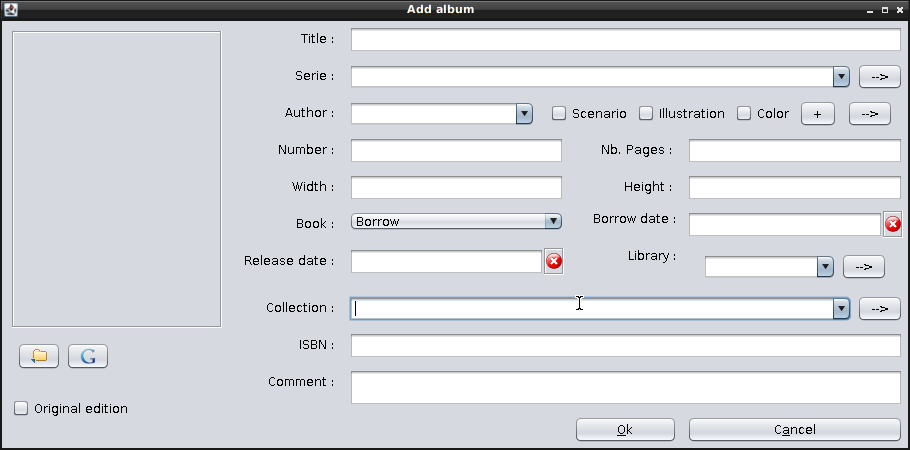
\includegraphics[width=300px]{figs/t3_ajoutAlbum.png} \\
A new system was built to allow user to use libraries and interact with it.
\end{center}
\end{block}
\end{frame}

\begin{frame}[Alert system]
\begin{block}{Alert system}
\begin{center}
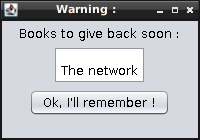
\includegraphics[width=100px]{figs/t3_warning.png} \\
At lunching, the application will check if you must give back albums in the next-days.
\end{center}
\end{block}
\end{frame}

\begin{frame}[E-mail import system]
\begin{itemize}
\item Able to import e-mail sent by the \emph{Android} application.
\pause \item Search \emph{ISBN}s numbers into e-mail.
\pause \item Information about \emph{ISBN} is search by the application into an online database.
\pause \item The album is automatically created.
\pause \item Users can choose from which library the book was borrowed, or editing informations about the album which was automatically imported.
\end{itemize}
\end{frame}

\subsection{Android application}
\begin{frame}
\begin{center}
\huge{Android application} \\ 
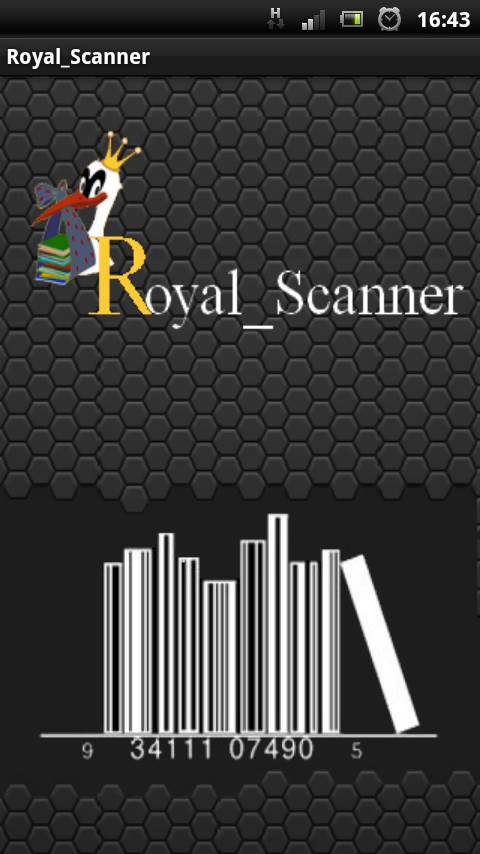
\includegraphics[width=90px]{figs/android_main.png}
\end{center}
\end{frame}

\begin{frame}[Scanner system]
\begin{itemize}
\item The application is able to scan a bar-code trough the camera.
\pause \item The application search the name of the album and display it to user.
\pause \item The scan can also be done with a group of albums. 
\end{itemize}
\begin{figure}[h!]
\uncover<2-> {
	\begin{minipage}[b]{0.4\linewidth}
	\centering 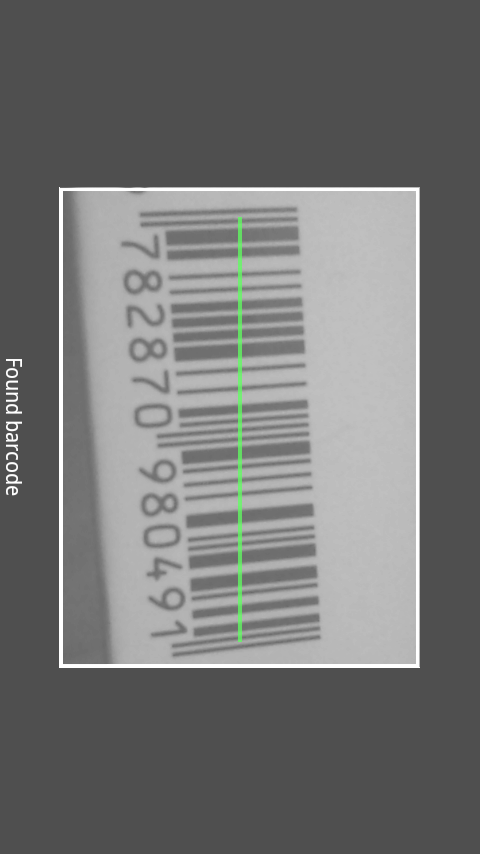
\includegraphics[width=60px, scale=1]{figs/android_isbn.png}
	\caption{Scan of an \emph{ISBN}}
	\end{minipage}
}
\uncover<3-> {
	\begin{minipage}[b]{0.4\linewidth}
	\centering 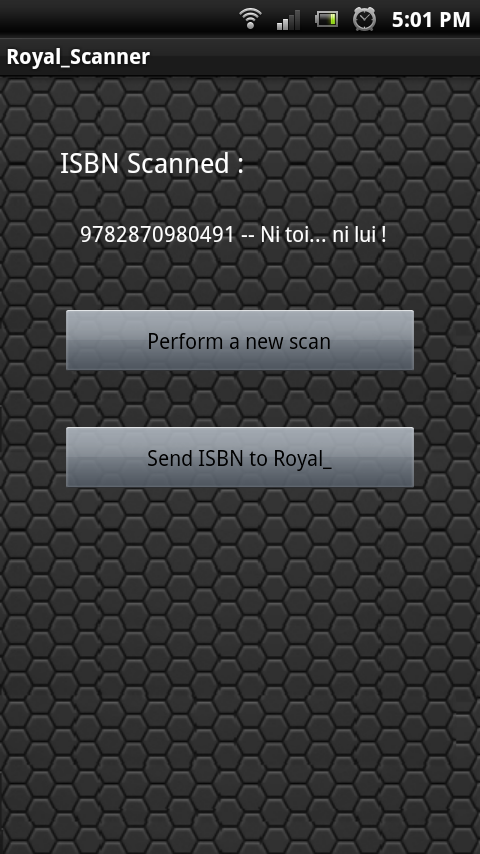
\includegraphics[width=60px, scale=1]{figs/android_name.png}
	\caption{A scanned album}
	\end{minipage}
}
\end{figure}
\end{frame}

\begin{frame}[Sending system and Database]
	\begin{block}{E-mail system}
		\begin{itemize}
			\item When \emph{ISBN}s are scanned, the application send it by e-mail, just in one click.
			\pause \item The user can, of course, make the e-mail address that he want.
		\end{itemize}
	\end{block}
	\pause
	\begin{block}{The database}
		\pause
		Album already scanned are register to prevent the user to scan an album twice.
	\end{block}
\end{frame}

\section{Difficulties}
\subsection{Libraries and API}

\begin{frame}
\begin{block}{Hibernate}
\begin{itemize}
\pause \item Still used into the project.
\pause \item Difficult to understand the concept.
\pause \item The diffucty was unexpected.
\end{itemize}
\end{block}
%\end{frame}


%\begin{frame}[Zxing]
\begin{block}{Zxing}
\begin{itemize}
\pause \item A \emph{Java} library to decode bar-code.
\pause \item Somes problem with \emph{Android} \pause : We're oblige to use an exteral apps.
\pause \item Thus : the library was dirrected inclued in the source code.
\end{itemize}
\end{block}
\end{frame}

\begin{frame}[JavaMail]
\begin{block}{JavaMail}
\begin{itemize}
\pause \item Sending e-mail is not very difficult with \emph{Android}.
\pause \item … But the gestion of e-mail is done by a other application \pause with allow user to modify the content of the e-mail.
\pause \item \textrightarrow We use \emph{JavaMail} instead of the default \emph{Android} application.
\end{itemize}
\end{block}
\end{frame}

\subsection{Integration  PC $\leftrightarrow$ Android}
\begin{frame}[Integration with PC]
\begin{block}{Integration of externals libraries}
\begin{itemize}
\pause \item Interoperability between the \emph{Android} and \emph{PC} application.
\pause \item For instance : e-mail libs used to twice applications are different.
\pause \item Integration of libraries into the project was litle difficult.
\end{itemize}
\end{block}
\end{frame}

\subsection{Technical tools}
\begin{frame}
\begin{block}{Eclipse}
\begin{itemize}
\pause \item A complex \emph{IDE} with a lot of fonctionality.
\pause \item Heavy deployement and many thinks to configure.
\pause \item Some time wasted in debuging because of Eclipse.
\end{itemize}
\end{block}
\pause 
\begin{block}{Git}
\begin{itemize}
\pause \item More complex that \emph{SVN}.
\pause \item Another phisosophy to understood. 
\pause \item Many tools to remembers how there work.
\end{itemize}
\end{block}
\end{frame}

\section{Bilan}

\begin{frame}
?
\end{frame}

\begin{frame}
?
\end{frame}

\section{Conclusion}
\begin{frame}
\begin{center}
\huge{Our feeling…}
\end{center}
\end{frame}

%\begin{frame}[The database]
%\begin{itemize}

\end{document}
